\newcommand{\HS}{Halting Segment\xspace}

\section{Halting Segment}\label{sec:halting-segment}

\begin{figure}[h!]
  \centering
  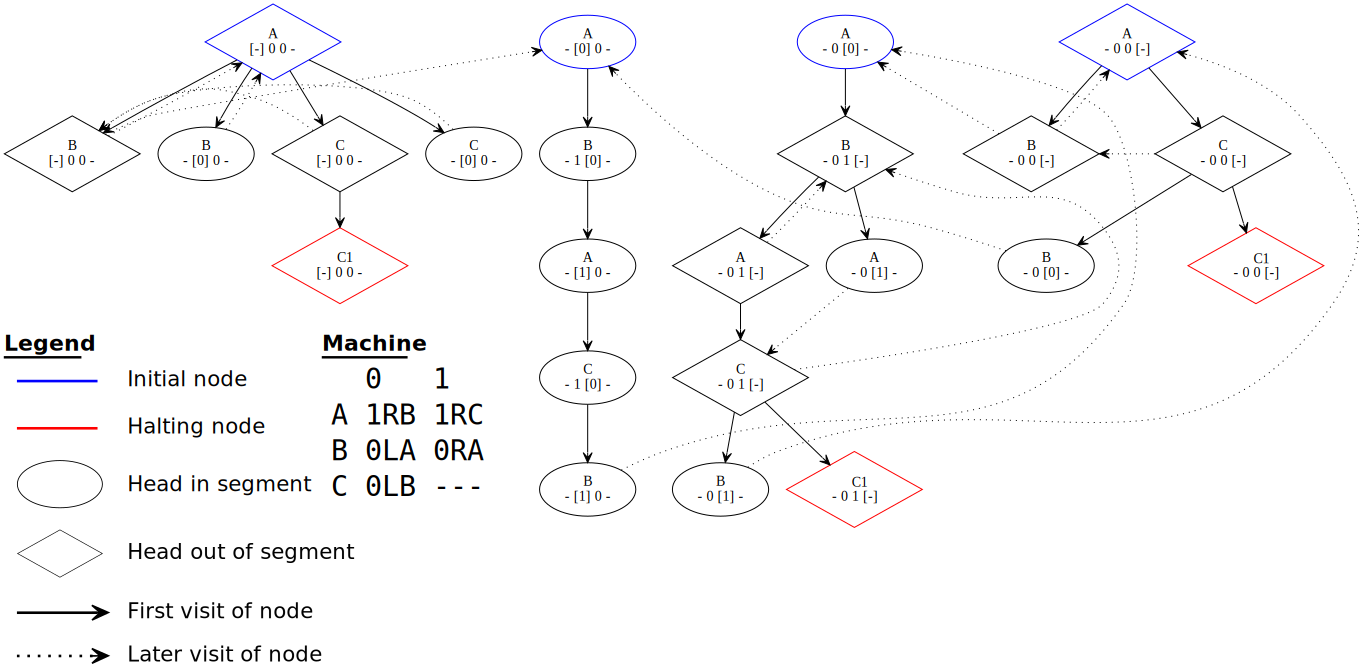
\includegraphics[width=1\textwidth]{halting-segment.pdf}
  \caption{\HS graph for the 3-state machine \url{https://bbchallenge.org/1RB1RC_0LA0RA_0LB---} and segment size 2, see Definition~\ref{def:hs-graph}. Nodes of this graph correspond to configurations of the machine on a finite segment (here, of size 2). In a node, the machine's head position is represented between brackets and the symbol \texttt{-} represents the outside of the segment (either to the left or to the right). Nodes where the machine's head is within the segment (circle shape) only one have child corresponding to the next step of the machine and nodes where the head is outside of the segment (diamond shape) may have multiple children corresponding to all the theoretically possible ways (deduced from the machine's transition table) that the machine can enter the segment back or continue to stay out of it. In order to improve readibility, edges that revisit a node are dotted. The machine presented here does not halt because the halting nodes (red outline) that are reachable from the initial nodes (blue outline) do not cover all the positions of the segment (there is no halting node for any of the two internal positions of the segment), see Theorem~\ref{th:hs:todo}. }\label{fig:hs}
\end{figure}

The idea of the \HS technique is to simulate a Turing machine on a finite segment of tape. When the machine leaves the segment in a certain state, we consider all the possible ways that it can re-enter the segment or stay out of it, based on the machine's transition table. For a given machine and segment size, this method naturally gives rise to a graph, the \HS graph (formally defined in Definition~\ref{def:hs-graph}).

Figure~\ref{fig:hs} gives the \HS graph of the 3-state machine\footnote{We chose a 3-state machine in order to have a graph of reasonable size.} \url{https://bbchallenge.org/1RB1RC_0LA0RA_0LB---} for segment size 2. Let's describe this graph in more details:

\begin{itemize}
  \item Nodes correspond to \textit{segment configurations}, i.e. the state in which the machine is together with the content of the segment and the position of the head in the segment (or outside of it). For instance, the leftmost node in blue and diamond shape in Figure~\ref{fig:hs} is \texttt{A [-] 0 0 -} which means that the machine is in state A, that the segment currently contains \texttt{0 0} and that the machine's head is currently outside of the segment, to the left of it.

  \item Initial nodes (blue outline) correspond to all sgement configurations that match the initial configuration of the machine (all-0 tape and state A), there are $n+2$ initial nodes with $n$ the size of the segment. Halting nodes (red outline) give the segment configurations where the machine has halted together with the halting transition that was used, for instance, in Figure~\ref{fig:hs}, the leftmost halting node \texttt{$\bot$ C1 [-] 0 0 -} signifies that the machine has halted ($\bot$), using halting transition \texttt{C1} (reading a 1 in state C), to the left of the segment which contains \texttt{0 0}.

  \item Nodes with a circle shape correspond to segment configurations where the tape's head is \textbf{inside} the segment. Such nodes only have one child which correspond to the next machine configuration.

  \item Nodes with a diamond shape correspond to segment configurations where the head is \textbf{outside} the segment, these nodes may have several children corresponding to all the ways that the head, in the current state, can stay outside of the segment or enter it back. For instance, the leftmost node in blue and diamond shape in Figure~\ref{fig:hs}, \texttt{A [-] 0 0 -}, has 4 children: \texttt{B [-] 0 0 -} and \texttt{B - [0] 0 -} and \texttt{C [-] 0 0 -} and \texttt{C - [0] 0 -}. This is because the transitions of the machine in state A are \texttt{1RB} and \texttt{1RC} and that the move \texttt{R} allows either to enter the segment back or to continue being out of it (if the head is far from the segment's left frontier). Note that the write symbol \texttt{1} of the transitions are ignored since we do not keep track of the tape outside of the segment.

  \item In order to increase the readability of Figure~\ref{fig:hs}, only one entrant edge for each node has been drawn with a solid line, corresponding to the first visit of that node in the particular order that the graph was visited. Later visits were drawn with a dotted line.
\end{itemize}

What is special about the \HS graph? We show in Theorem~\ref{th:hs} that if a machine halts, then, for all segment size, its \HS graph contains a set of halting nodes (red outline), for the same halting transition, that covers the entire segment and its outside, i.e. such that there is at least one such node per segment's position and outside of it (left and right). By contraposition, if there is no set of covering halting nodes for a halting transition, the machine does not halt. In Figure~\ref{fig:hs}, we deduce that machine \url{https://bbchallenge.org/1RB1RC_0LA0RA_0LB---} does not halt since the halting nodes of halting transition \texttt{C1} are \texttt{$\bot$ C1 [-] 0 0 -}, \texttt{$\bot$ C1 - 0 1 [-]} and \texttt{$\bot$ C1 - 0 0 [-]} which does not cover the entire segment (both internal segment postions are not covered).